\documentclass{article}

%% PAQUETES

% Paquetes generales
\usepackage[margin=2cm, paperwidth=210mm, paperheight=297mm]{geometry}
\usepackage[spanish]{babel}
\usepackage[utf8]{inputenc}
\usepackage{gensymb}

% Paquetes para estilos
\usepackage{textcomp}
\usepackage{setspace}
\usepackage{colortbl}
\usepackage{color}
\usepackage{color}
\usepackage{upquote}
\usepackage{xcolor}
\usepackage{listings}
\usepackage{caption}
\usepackage[T1]{fontenc}
\usepackage[scaled]{beramono}

% Paquetes extras
\usepackage{amssymb}
\usepackage{float}
\usepackage{graphicx}

%% Fin PAQUETES


% Definición de preferencias para la impresión de código fuente.
%% Colores
\definecolor{gray99}{gray}{.99}
\definecolor{gray95}{gray}{.95}
\definecolor{gray75}{gray}{.75}
\definecolor{gray50}{gray}{.50}
\definecolor{keywords_blue}{rgb}{0.13,0.13,1}
\definecolor{comments_green}{rgb}{0,0.5,0}
\definecolor{strings_red}{rgb}{0.9,0,0}

%% Caja de código
\DeclareCaptionFont{white}{\color{white}}
\DeclareCaptionFont{style_labelfont}{\color{black}\textbf}
\DeclareCaptionFont{style_textfont}{\it\color{black}}
\DeclareCaptionFormat{listing}{\colorbox{gray95}{\parbox{16.78cm}{#1#2#3}}}
\captionsetup[lstlisting]{format=listing,labelfont=style_labelfont,textfont=style_textfont}

\lstset{
	aboveskip = {1.5\baselineskip},
	backgroundcolor = \color{gray99},
	basicstyle = \ttfamily\footnotesize,
	breakatwhitespace = true,   
	breaklines = true,
	captionpos = t,
	columns = fixed,
	commentstyle = \color{comments_green},
	escapeinside = {\%*}{*)}, 
	extendedchars = true,
	frame = lines,
	keywordstyle = \color{keywords_blue}\bfseries,
	language = Oz,                       
	numbers = left,
	numbersep = 5pt,
	numberstyle = \tiny\ttfamily\color{gray50},
	prebreak = \raisebox{0ex}[0ex][0ex]{\ensuremath{\hookleftarrow}},
	rulecolor = \color{gray75},
	showspaces = false,
	showstringspaces = false, 
	showtabs = false,
	stepnumber = 1,
	stringstyle = \color{strings_red},                                    
	tabsize = 2,
	title = \null, % Default value: title=\lstname
	upquote = true,                  
}

%% FIGURAS
\captionsetup[figure]{labelfont=bf,textfont=it}
%% TABLAS
\captionsetup[table]{labelfont=bf,textfont=it}

% COMANDOS

%% Titulo de las cajas de código
\renewcommand{\lstlistingname}{Código}
%% Titulo de las figuras
\renewcommand{\figurename}{Figura}
%% Titulo de las tablas
\renewcommand{\tablename}{Tabla}
%% Referencia a los códigos
\newcommand{\refcode}[1]{\textit{Código \ref{#1}}}
%% Referencia a las imagenes
\newcommand{\refimage}[1]{\textit{Imagen \ref{#1}}}


\begin{document}

% Inserción del título, autores y fecha.
\title{\Large 75.42 Taller de Programación I \\ 
	  \medskip\Huge Informe: Ejercicio N° 2  \\
	  \bigskip\Large\textit{``Procesador de caminos mínimos por Dijkstra''}}
\date{}
\maketitle




% INTRODUCCIÓN
\section{Introducción}
	
	A causa de los constantes problemas de tráfico de red que posee la empresa ITCorp S.A., se nos ha solicitado el desarrollo de un módulo para el cálculo de routeo entre PCs a través de routers contenidos en una red para, de esta manera, poder configurar de forma manual el routeo entre PCs y así minimizar el recorrodo de los paquetes de datos.
	\par
	Para resolver el problema del camino de ruteo entre dos PCs, se requiere el uso el \textit{Algoritmo de Dijkstra}, el cual tiene como objetivo el cálculo del camino mínimo entre dos nodos.
	\par
	Detalles mas precisos de la problemática y de las condiciones preestablecidas se pueden encontrar en el enunciado del ejercicio\footnote{Se ha evitado hacer un relevamiento de la totalidad de la información que nos fue conferida, de manera de poder mantener el foco del informe en la forma en que se ha encarado la solución del problema.}.
\bigskip




% CONSIDERACIONES DE DISEÑO
\section{Consideraciones de diseño}

	Para la correcta implementación de la solución fue necesario plantear y establecer cómo se debería comportar el sistema ante ciertas situaciones que no fueron especificadas en el enunciado del problema. A continuación se listan las contemplaciones instauradas:

\begin{itemize}
	\itemsep=3pt \topsep=0pt \partopsep=0pt \parskip=0pt \parsep=0pt

	\item Se supone que, en el caso de utilizar un archivo como la fuente de especificaciones de routeo, este se encuentra estrictamente dispuesto con el formato preestablecido en el enunciado del ejercicio, dejando en el usuario la responsabilidad de asegurar el cumplimiento de esta norma;

	\item En caso de no poder ser abierto el archivo, se lanzará un mensaje de error a la salida estándar, y el programa retornará 0;

	\item Los pesos de los caminos o conexiones entre dispositivos de la red son estrictamente enteros;

	\item El nombre de un host o router en la red es único, así como también, obviamente, su IP;

	\item El archivo de especificación de ruteo contiene dispuestas las secciones en un orden fijo, definiendose primero los hosts, luego los dispositivos y por último los ruteos o conexiones entre estos.

\end{itemize}
\smallskip




% DISEÑO
\section{Diseño}

	Como creemos que la escalabilidad de un sistema (en este caso del programa) es muy importante, es que se ha decidido modularizar consistentemente ciertas partes que conforman las especificaciones, de manera de permitirnos, en un futuro, agregar o mejorar más fácilmente el funcionamiento del mismo. Para lograr este propósito se hará uso, entre otras cosas, de TDAs y estructuras.
	\par
	En los apartados que siguen pondremos la atención en aquellos aspectos de la implementación que pueden ser relevantes a causa de su complejidad o particularidad. En estos se describen los inconvenientes que presentan y la forma en que fueron resueltos.
\bigskip



% DISEÑO - Procesamiento de especificaciones de routeo
\subsection{Procesamiento de especificaciones de routeo}

	Una de las cuestiones mas significativas se relaciona con cómo el programa manejará la información provista por el usuario, de manera tal de lograr un procesamiento que además de ser eficiente, se encuentre coherentemente estructurado. Es decir, deseamos agrupar la información que se encuentra ligada a algún ente abstracto y así conseguir una división más profunda del problema.
	\par
	Se ha resuelto entonces, dividir la especificación ingresada en dos estructuras: \textit{host} y \textit{device}. Al inicio del programa, se parsearán los datos y se crearán hosts y devices de acuerdo a estas estructuras. Cabe resaltar que cada host sabe a que dispositivo se encuentra conectado ya que posee registro del nombre de este.
	\par
	Esta forma de organización nos permite crear un grafo que representará a la red, pero que sólo va a constar de datos de tipo \textit{device} como vértices o nodos. Las aristas de este simbolizan las conexiones entre los dispositivos, y son cargadas a medida que se parsea cada entrada de \textit{routes}. El grafo resultante es el que será utilizado posteriormente para el cálculo de caminos mínimos.
	\par
	Una vez procesado el grafo con el \textit{Algoritmo de Dijkstra}, se utilizan los hosts creados previamente para poder localizar el punto de partida de los paquetes de datos y los distintos puntos de destino de estos últimos. Finalmente, se envían a la salida estándar los caminos desde el origen hacia los demás hosts.
\bigskip



% DISEÑO - Librería dijkstra.h
\subsection{Librería \textit{dijkstra.h}}

	Por razones que aquí expondremos, hemos creado una librería en la cual se agrupan distintos tipos de funciones relacionadas con el cálculo de caminos mínimos. La función mas destacable de esta librería es \textit{dijkstra\_caminos\_minimos()}, quien es la encargada de aplicar el algoritmo de Dijkstra a un grafo de nodos no aislados. Dicha función devolverá una lista de resultados. Lo particular de esto es que dichos resultados no serán directamente computables por el usuario que utilice la función. Para poder acceder a ellos se deberá hacer uso de las otras funciones que provee la librería.
	\par
	Esta decisión de implementación aporta la ventaja de que el usuario solo necesitará llamar a la función que calcula los caminos mínimos una única vez para cierto nodo origen. Luego, como ya se tienen los resultados, simplemente se pasarán estos últmos a las funciones de la librería de acuerdo a que es lo que se necesite obtener de ellos.
	\par
	Un detalle final a tener en cuenta es que, para evitar pérdidas de memoria, es necesario que el usuario, al terminar de utilizar la lista de resultados, haga uso de la función de destrucción de resultados de la librería para poder liberar la memoria utilizada por estos.
\bigskip


% DISEÑO - Librería dijkstra.h - Función de criterio de selección 
% de caminos
\subsubsection{Función de criterio de selección de caminos}

	
	Si se observa el código fuente de la librería, podrá notarse que la función \textit{dijkstra\_caminos\_minimos()} además de recibir como parámetros dos listas del TDA \textit{Lista}, recibe un puntero a una función declarada como
\bigskip

{\ttfamily\footnotesize
\indent int criterio\_seleccion(lista\_dato\_t, lista\_dato\_t).\\}

	\par
	Esta se utiliza dentro del algoritmo de Dijkstra en los casos de ambigüedad que surgen cuando a un nodo se llega por dos caminos diferentes con igual longitud al origen. Es allí donde el criterio de selección definido por el usuario es utilizado, delegando la responsabilidad de la elección del camino a quien utilice la función de cálculo de caminos mínimos.
	\par
	La función que debe pasar el usuario por parámetro, recibe los dos vértices desde los cuales se llegó al nodo actual, que es en donde se genera la ambigüedad de caminos. Nótese que, como el algoritmo de Dijkstra no sabe de que tipo son en realidad los vértices del grafo, entonces pasa a la función los dos nodos con el tipo definido para las listas, que, como se detallará en la \textit{Sección 3.4}, son \textit{void*}. Para poder utilizar estos dos datos recibidos por parámetro, el usuario deberá castearlos dentro de su función al tipo de dato con el cual fueron creados inicialmente, es decir, al tipo con el cual fueron ingresados en el grafo.
	\par
	Por último, la función deberá devolver un valor entero menor a cero si se desea elegir el camino del primer parámetro ó un valor entero mayor a cero si se desea elegir el camino del segundo parámetro.
\bigskip



% DISEÑO - TDA Grafo
\subsection{TDA \textit{Grafo}}

	Dejando de lado la exposición de las primitivas definidas para el TDA \textit{Grafo}, focalizaremos nuestra atención en como es que fue implementado el núcleo del TDA.
	\par
	Es sabido que dos posibles formas de construir un grafo son a través de una \textit{matriz de adyacencia} o de una \textit{lista de adyacencia}. En este punto, hemos considerado que el número de vértices (simbolizando dispositivos de la red) no es significativamente grande, es decir, el grafo estará en la mayoría de los casos escasamente poblado. Además, hemos estimado que el grafo generalmente será medianamente disperso, significando esto que constará de una cantidad de aristas no numerosa. Dados estos supuestos, se ha decidido que el grafo sea implementado a partir de una variación de la \textit{lista de adyacencia}.
\bigskip


% Figura 1
\begin{figure}[h]
	\centering
	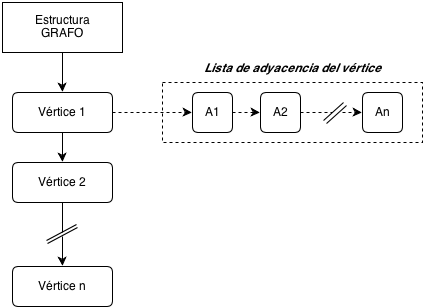
\includegraphics[width=0.55959299\textwidth]{images/diagrama01.png}
	\medskip
	\caption{Diagrama del núcleo del grafo implementado.}
\end{figure}
\medskip
	

	En la \textit{Figura 1} se muestra un diagrama en el que se ilustra como es que está construido el núcleo del grafo. En primer lugar, se puede observar la estructura \textit{Grafo}, la cual posee un puntero al primer vértice del grafo (en caso de existir). Al ir agregando vértices, estos se enlazarán entre sí con la forma de una lista enlazada mediante punteros. Por otro lado, cada vértice posee un puntero a una lista de adyacencia propia. En esta lista se van almacenando punteros a los vértices adyacentes del grafo.
\bigskip



% DISEÑO - TDA Lista
\subsection{TDA \textit{Lista}}

	La última problemática que se considera importante destacar es la que surge con los TDAs implementados, particularmente con el TDA \textit{Lista}, la cual implementa un tipo abstracto de datos para las listas simplemente enlazadas. Los usuarios que usen los TDAs pueden definir el tipo de dato que van a almacenar, agregando en el archivo donde se incluye el header de cada uno de ellos las líneas que se especifican en los mismos, y que por ejemplo, para el caso de uso de \textit{Lista} con datos de tipo \textit{integer} resultan ser
\bigskip

	{\ttfamily\footnotesize
\indent \#define LISTA\_DATO\_T\\
\indent typedef int lista\_dato\_t;\\}

	La desventaja de esto se presenta cuando se es necesario utilizar mas de una lista a la vez y que en todas se almacenen distintos tipos de datos, ya que, al realizar una definición como la expuesta anteriormente, nos estamos limitando a que todas las listas a crear permitan solamente datos de dicho tipo. 
	\par
	Desafortunadamente nos ha sido inevitable el uso de múltiples listas, optándose así por una de las tantas soluciones existentes de manera de lograr apaciguar el problema. En el TAD \textit{Lista}, por defecto se definen como \textit{void*} los elementos a almacenar. Por lo tanto, se ha decido mantener esta determinación de implementación y, para cada lista, al momento de insertar un elemento, se requerirá un casteo previo a \textit{lista\_dato\_t}. Al leerlo o sacarlo de la lista, por ende, será necesario castearlo a su tipo original.
\bigskip




% ESQUEMA DEL DISEÑO
\section{Esquema del diseño}

	A continuación, en la \textit{Figura 2}, se ilustra el diagrama de flujo que representa la secuencia de ejecución de los distintos procesos que se deben llevar a lo largo de cada parte del programa.

\newpage
% Figura 2
\begin{figure}[h]
	\centering
	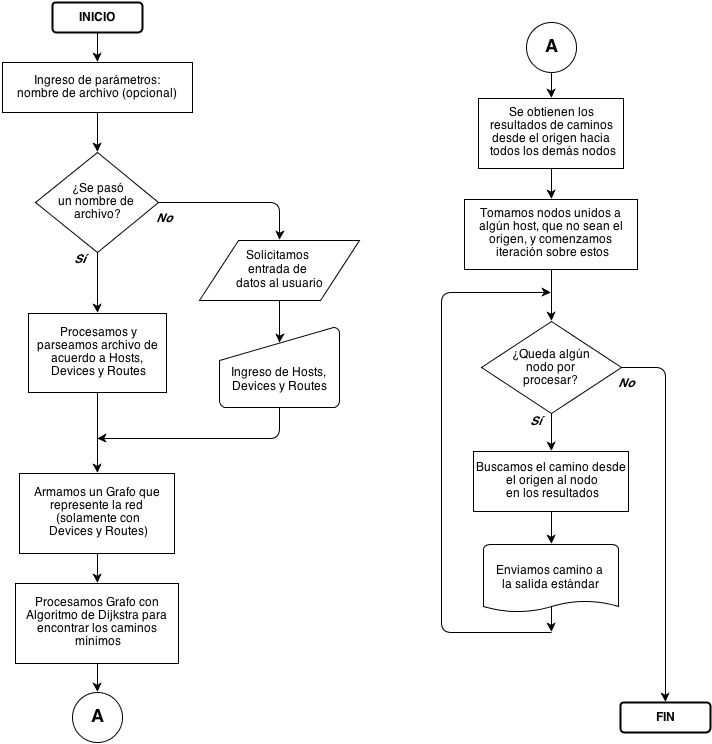
\includegraphics[width=0.968976\textwidth]{images/diagrama02.png}
	\medskip
	\caption{Diagrama de flujo representativo de la solución.}
\end{figure}


\end{document}
